%==============================================================================
% Sjabloon onderzoeksvoorstel bachelorproef
%==============================================================================
% Gebaseerd op LaTeX-sjabloon ‘Stylish Article’ (zie voorstel.cls)
% Auteur: Jens Buysse, Bert Van Vreckem
%
% Compileren in TeXstudio:
%
% - Zorg dat Biber de bibliografie compileert (en niet Biblatex)
%   Options > Configure > Build > Default Bibliography Tool: "txs:///biber"
% - F5 om te compileren en het resultaat te bekijken.
% - Als de bibliografie niet zichtbaar is, probeer dan F5 - F8 - F5
%   Met F8 compileer je de bibliografie apart.
%
% Als je JabRef gebruikt voor het bijhouden van de bibliografie, zorg dan
% dat je in ``biblatex''-modus opslaat: File > Switch to BibLaTeX mode.

\documentclass{voorstel}

\usepackage{lipsum}
\usepackage{float}

%------------------------------------------------------------------------------
% Metadata over het voorstel
%------------------------------------------------------------------------------

%---------- Titel & auteur ----------------------------------------------------

% TODO: geef werktitel van je eigen voorstel op
\PaperTitle{Geautomatiseerd parsen van systeem logs}
\PaperType{Onderzoeksvoorstel Bachelorproef 2020-2021} % Type document

% TODO: vul je eigen naam in als auteur, geef ook je emailadres mee!
\Authors{Marbod Naassens\textsuperscript{1}} % Authors
\CoPromotor{Geert De Paep\textsuperscript{2} (Exitas)}
\affiliation{\textbf{Contact:}
  \textsuperscript{1} \href{mailto:marbod.naassens@student.hogent.be}{marbod.naassens@student.hogent.be};
  \textsuperscript{2} \href{mailto:Geert.DePaep@exitas.be}{Geert.DePaep@exitas.be};
}

%---------- Abstract ----------------------------------------------------------

\Abstract{
    Binnen deze bachelorproef wordt er dieper ingegaan op één van de processen binnen anomaliedetectie van systeem en applicatie logfiles. Logfiles zijn bestanden die de continuïteit van een systeem of applicatie weergeven. Door deze te observeren, kunnen fouten binnen het systeem of de applicatie naar boven komen. De anomaliedetectie van deze files helpt ons om sneller fouten te detecteren en op te lossen. Deze bachelorproef zal binnen anomaliedetectie kijken naar de verschillende parsing methodes voor deze logfiles. Parsingmethodes zijn methodes om een bestand te organiseren en leesbaarder te maken. De logfiles op zich zijn niet zeer leesbaar of analyseerbaar, maar door deze parsingmethodes worden de logfiles meer gestructureerd, aldus makkelijker om te analyseren, waardoor anomaliedetectie mogelijk wordt. Om specifieker te zijn zal dit onderzoek vooral kijken naar verschillende reeds bestaande log parsingmethodes (automatisch en niet-automatisch) en deze zullen worden vergeleken om te achterhalen wat de best-practices methodes en parsing technologieën zijn.
    Experimenten zullen uitgevoerd worden om de hypothese vanuit de paper `Tools and Benchmarks for Automated Log Parsing` te onderzoeken. Verder zullen we experimenteren met parsers die niet zijn opgenomen in de reeds vernoemde paper. In dit werk zal omschreven worden welke parsingmethodes geprefereerd worden in een real-time setting en waar men moet op letten bij het parsen van systeem logs. Er zal ook vermeld worden welke technologieën er beschikbaar zijn voor log parsing en welke binnen deze technologieën de laagste foutenmarge en de laagste tijdscomplexiteit zullen bevatten. 
    Van deze bachelorproef wordt verwacht dat deze voor volgend onderzoek, of voor opbouwend onderzoek binnen anomaliedetectie van logfiles, een informatiebron kan zijn voor het belang van log parsing en de verschillende onderdelen binnen log parsing. Ook wordt er verwacht dat deze bachelorproef een duidelijk antwoord zal geven op de vraag wat de beste parsingmethode is binnen systeem logs in een real-time setting. De assumptie is dat, zoals in de bovenvernoemde paper, `Drain` als beste en meest efficiënte parsingtool naar boven zal komen.
    Dit werk is zeer actueel, want elke dag komen we in contact met verschillende applicaties en systemen. Dit betekent dat naar de toekomst toe er een exponentiële stijging zal zijn in het aantal logfiles. Van dit werk wordt vooral verwacht dat het een duidelijke leidraad zal zijn voor de keuze van parsingmethodes binnen anomaliedetectie, i.e. een duidelijke weergave van welke parsingmethode men het best gebruikt en verder wordt verwacht dat het een basis zal vormen voor verder onderzoek naar parsingmethodes en de ontwikkeling van nieuwe technologieën.
}

%---------- Onderzoeksdomein en sleutelwoorden --------------------------------
% TODO: Sleutelwoorden:
%
% Het eerste sleutelwoord beschrijft het onderzoeksdomein. Je kan kiezen uit
% deze lijst:
%
% - Mobiele applicatieontwikkeling
% - Webapplicatieontwikkeling
% - Applicatieontwikkeling (andere)
% - Systeembeheer
% - Netwerkbeheer
% - Mainframe
% - E-business
% - Databanken en big data
% - Machineleertechnieken en kunstmatige intelligentie
% - Andere (specifieer)
%
% De andere sleutelwoorden zijn vrij te kiezen

\Keywords{Machineleertechnieken. Logs --- Parsing --- Anomaliedetectie --- Python} % Keywords
\newcommand{\keywordname}{Sleutelwoorden} % Defines the keywords heading name

%---------- Titel, inhoud -----------------------------------------------------
\usepackage{biblatex} 

\begin{document}
\flushbottom % Makes all text pages the same height
\maketitle % Print the title and abstract box
\tableofcontents % Print the contents section
\thispagestyle{empty} % Removes page numbering from the first page

%------------------------------------------------------------------------------
% Hoofdtekst
%------------------------------------------------------------------------------

% De hoofdtekst van het voorstel zit in een apart bestand, zodat het makkelijk
% kan opgenomen worden in de bijlagen van de bachelorproef zelf.
%---------- Inleiding ---------------------------------------------------------

\section{Introductie} % The \section*{} command stops section numbering
\label{sec:introductie}
Logfiles zijn belangrijk binnen verschillende applicaties en systemen. Ze geven de werking van een applicatie weer en kunnen gebruikt worden voor het vinden van fouten binnen de applicatie. In de huidige samenleving werkt men elke dag met verschillende computerapplicaties en software. Men wil dat deze applicaties en software efficiënt werken en snel alledaagse problemen oplossen. Mocht er zich een softwareprobleem voordoen, wil men dan ook dat dit snel wordt opgelost door de applicatieontwikkelaars. Binnen deze context valt dan het analyseren van de logbestanden om zo snel mogelijk deze fouten te vinden of om toekomstige fouten te voorkomen. Het automatiseren van anomaliedetectie, dit zijnde het detecteren van fouten of afwijkingen binnen een applicatie of software systeem, binnen systeem en applicatielogs is dus iets waarbinnen IT veel waarde aan vasthangt. 
Voordat men aan anomaliedetectie kan beginnen, moet men eerst de logfiles kunnen implementeren. Deze files moeten gestructureerd worden zodat het duidelijker wordt wat de inhoud van de logfiles is, zodat men ook de essentie van de logfiles kan bepalen. Hiervoor is parsing nodig van de logs. De parsing zorgt voor structuur en duidelijke grenzen zodat men makkelijker de logfiles kan analyseren. 
Als men dit handmatig zou moeten doen, in een tijd waar er terabytes aan data zich bevinden in de logfiles, dan zou dit niet enkel tijdconsumerend zijn, maar ook zeer onderhevig aan menselijke fouten. 
Het geautomatiseerd parsen van systeem logs is dus een cruciaal deel bij anomaliedetectie binnen de logs en dit is een belangrijk deel bij het onderhouden van applicaties.
Deze bachelorproef zal dieper ingaan op het geautomatiseerd parsen van systeem logs. De analyse van systeemlogs wordt toegepast voor anomaliedetectie, probleem indentificatie, gebruiksanalyse, etc.. In deze bachelorproef is het de bedoeling om een aantal log parsers te onderzoeken en de werking ervan te analyseren om zo een log parser te vinden die het best kan gebruikt worden in een real-time setting.

%---------- Stand van zaken ---------------------------------------------------

\section{State-of-the-art}
\label{sec:state-of-the-art}
Ten eerste is dit onderzoek gebasseerd op een recent uitgebrachte paper~\autocite{TBA2019}. In dit onderzoek kwam men tot de conclusie dat `Drain` de meest accurate en performante log parser is. Dit blijkt uit meerdere testen die zijn uitgevoerd met 16 verschillende logs, waaruit random 2000 lijnen werden genomen om de parser op toe te passen. Dit werd gedaan omdat anders het parsen te lang duurde door de grootte van de logfiles. Drain bleef ook geprefereerd nadat men een tweede onderzoek uitvoerde met maar 3 logsets, zijnde: Android, HDFS en BGL en een selectie parsers, namelijk: MoLFI\autocite{messaoudi2018search}, Spell\footnote{Streaming Parsing of System Event Logs}\autocite{du2016spell}, LenMa\footnote{Length Matters}\autocite{shima2016length}, IPLoM\footnote{Iterative Partitioning Log Mining}\autocite{makanju2009clustering}, AEL\footnote{Abstracting Execution Logs}\autocite{jiang2008abstracting}, en Drain\autocite{he2017drain}. In het tweede onderzoek werd er uit de logs random 300KB tot 1GB gekozen om te zien wat het verschil is van de output van de parsers op een kleine dataset en een grote dataset en hoe performant dit zou blijven.
Echter is het wel belangrijk om te melden dat op het einde van de paper men ook vermeldt dat verder onderzoek duidelijk nodig is door de beperktheid van de parsers.
Het onderzoek zal ten eerste beperkt worden tot een real-time setting, dit omdat deze bachelorproef een basis voor de analyse en anomaliedetectie van logfiles moet vormen. Hierbij is tijd een belangrijke factor. 

Andere beperkingen die in het onderzoek zullen opgelegd worden, zijn:
\begin{itemize}
    \item Een parser moet een goede parsing opleveren, i.e. een leesbare en duidelijk analyseerbare parsing.
    \item Een gekozen parser moet ‘ongesuperviseerd’ kunnen getraind worden.
    \item Een parser moet snel werken. Hiermee wordt een tijdscomplexiteit bedoeld die hoogstens lineair is in het aantal karakters en aantal verschillende parserboodschappen.
\end{itemize}

Het onderzoeken van de resultaten van de paper `Tools and Benchmarks for Automated Log Parsing`\\ ~\autocite{TBA2019}, is niet het enige deel van deze bachelorproef. Het is ook de bedoeling om deze paper uit te breiden door een breder onderzoek te voeren. Dit zal worden bereikt door het introduceren van nieuwe datasets en nieuwe log parsers die nog niet werden vernoemd in de bovenstaande paper.

Op basis van `LogLens: A Real-time Log Analysis System` ~\autocite{LogLens2018}, is de keuze gemaakt om elastic.co's LogStash te gebruiken als extra niet voorgedefinieerde log parser. In deze paper gaat men ook dieper in op een zelfgemaakt systeem dat 41 keer sneller dan LogStash zou functioneren en dus efficiënter is voor real-time voorbeelden. Echter is er omtrent het gebruik en downloaden van LogLens geen verdere info beschikbaar.
Bij verder onderzoek zijn volgende aanvullende log parsers gekozen:

\begin{itemize}
    \item XPLG's PortX\footnote{https://www.xplg.com/port-x-log-parser/}
    \item Solarwind's Security Event Manager log parser\footnote{https://www.solarwinds.com/security-event-manager/use-cases/log-parser-tool}
    \item  GoAccess\footnote{https://goaccess.io/ , Log Analysis tool met eigen log parser}
    \item  Datadog's FluentBit \footnote{https://www.datadoghq.com/ , Log Analysis tool met eigen log parser}
    \item NuLog\footnote{https://github.com/nulog/nulog , Open source log parser met ~\autocite{TBA2019} als basis}
    \item LogParse\footnote{https://github.com/NetManAIOps/LogParse}
\end{itemize}

Hierbij moet wel vermeld worden dat NuLog en LogParse beide gevonden zijn via de literatuurstudie. Dit zijn open source log parsers die zijn gecreëerd voor hun respectievelijke papers, voor NuLog was dit de paper `Self-Supervised Log Parsing` ~\autocite{SSLP2020} en voor LogParse was dit de paper `LogParse: Making Log Parsing Adaptive through Word Classification` ~\autocite{LogParse2020}.
Deze onderzoeken lopen ook gelijkaardig met het onderzoek van deze bachelorproef, maar afgebakend voor hun eigen domein. Zo is NuLog onderzocht geweest met een focus op gesuperviseerd logparsen en is LogParse onderzocht geweest met een focus op het adaptiever maken van logparsing. Deze is dan ook opgesteld op basis van andere log parsers ~\autocite{LogParse2020}.

Bij dit onderzoek wordt de vraag gesteld: 'Wat is de snelste log parser die een duidelijke en analyseerbare parsing opleverd voor loganomaliedetectie en die ongesuperviseerd getraind kan worden in een real-time setting?'. 

% Voor literatuurverwijzingen zijn er twee belangrijke commando's:
% \autocite{KEY} => (Auteur, jaartal) Gebruik dit als de naam van de auteur
%   geen onderdeel is van de zin.
% \textcite{KEY} => Auteur (jaartal)  Gebruik dit als de auteursnaam wel een
%   functie heeft in de zin (bv. ``Uit onderzoek door Doll & Hill (1954) bleek
%   ...'')


%---------- Methodologie ------------------------------------------------------
\section{Methodologie}
\label{sec:methodologie}

Dit onderzoek, zoals reeds eerder vermeld, wordt opgebouwd op basis van een reeds gevoerd onderzoek ~\autocite{TBA2019}. Hierbij wordt gebruik gemaakt van de opensource software die ter beschikking wordt gesteld door dit eerder onderzoek. Op basis hiervan kunnen eigen aanpassingen gemaakt worden en eigen extra log parsers toegevoegd worden. Deze opensource library wordt aan de hand van dependencies toegevoegd aan Python, gegeven dat Python ook een handige tool is voor het analyseren van data zal het onderzoek van deze bachelorproef dan ook volledig in Python worden uitgevoerd. Tools zoals FluentBit en GoAccess hebben hun eigen platform en voor de analyse van hun efficiëntie en accuraatheid zal dan ook hun eigen platform gebruikt worden.

In Python en op de andere platformen zullen simulaties worden aangemaakt van datasets die geparsed zullen worden en deze zullen manueel geanalyseerd worden voor accuraatheid. Hierbij zullen de datasets wel moeten beperkt worden. In een tweede stap kan verder gegaan worden met grotere datasets, maar dit zal moeilijker zijn om manueel de accuraatheid te gaan bepalen. Echter geeft dit ons wel een duidelijker overzicht van de snelheid en efficiëntie van deze parsers.

%---------- Verwachte resultaten ----------------------------------------------
\section{Verwachte resultaten}
\label{sec:verwachte_resultaten}

Op basis van de literatuurstudie kan al een deelgrafiek weergeven worden voor de verwachte resultaten (Figuur 1). Deze grafiek kan men vinden in de paper `Tools and Benchmarks for Automated Log Parsing`. De grafiek geeft de verschillende log parsers weer met hun respectievelijke accuraatheid bij de verschillende datasets.
In het onderzoek van deze bachelorproef komen er nog meerdere parsers bij en zullen we de grafiek aanvullen met de resultaten hiervan. Uit literatuuronderzoek zou bovendien blijken dat LogStash een kandidaat is om in een real-time setting boven Drain uit te blinken. Dit zullen we evalueren in ons onderzoek.

\begin{figure}[H]
    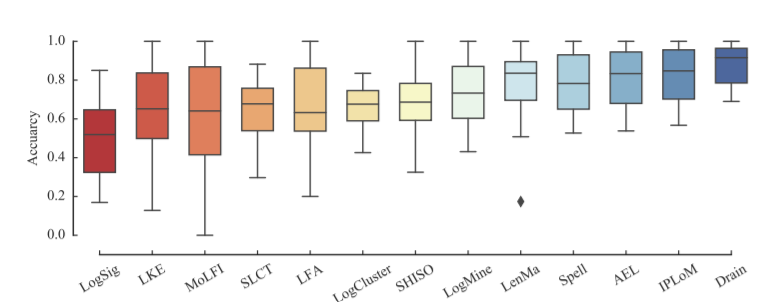
\includegraphics[width= \linewidth]{graph.png}
    \caption{Grafiek uit de paper `Tools and Benchmarks for Automated Log Parsing`~\autocite{TBA2019}}
\end{figure}

%---------- Verwachte conclusies ----------------------------------------------
\section{Verwachte conclusies}
\label{sec:verwachte_conclusies}

De nulhypothese van dit onderzoek is als volgt, op basis van literatuuronderzoek:\\
Drain zal naar boven komen als de meest geschikte log parser vanwege zijn efficiëntie en accuraatheid.

Het is de bedoeling om deze hypothese te confirmeren of te verwerpen en te zoeken naar een betere oplossing, dit zijnde een andere log parser, voor het parsen in een realtime setting omdat qua snelheid van parsing er nog altijd een grote beperking heerst zelfs met Drain.



%------------------------------------------------------------------------------
% Referentielijst
%------------------------------------------------------------------------------
% TODO: de gerefereerde werken moeten in BibTeX-bestand ``voorstel.bib''
% voorkomen. Gebruik JabRef om je bibliografie bij te houden en vergeet niet
% om compatibiliteit met Biber/BibLaTeX aan te zetten (File > Switch to
% BibLaTeX mode)

\phantomsection
\printbibliography[heading=bibintoc]

\end{document}
